\documentclass{jib}
\newlength{\platz}
\setlength{\platz}{15pt}
\RequirePackage{listings}
\lstset{%
  basicstyle=\ttfamily,
  fontadjust,
  flexiblecolumns=true,
  frame=L,
  xleftmargin=15pt,
  framesep=5pt,
  emphstyle=\rmfamily\itshape}

\usepackage{pdfpages}

%%%%%%%%%%%%%%%%%%%%%%%%%%%%%%%%%%%%%%%%%%%%%%%%%%%%%%%%%%
% JIB Header/Footer
%%%%%%%%%%%%%%%%%%%%%%%%%%%%%%%%%%%%%%%%%%%%%%%%%%%%%%%%%%
\jibvolume{XX} % insert volume
\jibissue{X}   % insert issue
\jibpages{XXX} % insert article ID
\jibyear{XXXX} % insert year
\makeHeaderFooter{} % leave as is
%%%%%%%%%%%%%%%%%%%%%%%%%%%%%%%%%%%%%%%%%%%%%%%%%%%%%%%%%%

\begin{document}

%%%%%%%%%%%%%%%%%%%%%%%%%%%%%%%%%%%%%%%%%%%%%%%%%%%%%%%%%%
%
% Title Page
%
%%%%%%%%%%%%%%%%%%%%%%%%%%%%%%%%%%%%%%%%%%%%%%%%%%%%%%%%%%

\begin{jibtitlepage}

\jibtitle{Systems Biology Markup Language (SBML) Level~2:\\
Structures and Facilities for Model Definitions}

\jibauthor{%
  Michael Hucka\iref{caltech},
  Frank T. Bergmann\iref{caltech},
  Andreas Dr\"{a}ger\iref{ucsd},
  Stefan Hoops\iref{vtech},\\
  Sarah M. Keating\iref{ebi},
  Nicolas Le~Nov\`{e}re\iref{bi},
  Chris J. Myers\iref{uu},
  Brett G. Olivier\iref{vu},
  Sven Sahle\iref{uh},
  James C. Schaff\iref{uchc},
  Lucian P. Smith\iref{uw},
  Dagmar Waltemath\iref{rostock},
  Darren J. Wilkinson\iref{newcastle}%
}

\addjibinstitution{caltech}   {California Institute of Technology, USA}
\addjibinstitution{ucsd}      {University of California, San Diego, USA}
\addjibinstitution{vtech}     {Virginia Bioinformatics Institute, USA}
\addjibinstitution{ebi}       {European Bioinformatics Institute, UK}
\addjibinstitution{bi}        {Babraham Institute, UK}
\addjibinstitution{uu}        {University of Utah, USA}
\addjibinstitution{vu}        {VU University Amsterdam, The Netherlands}
\addjibinstitution{uh}        {University of Heidelberg, Germany}
\addjibinstitution{uchc}      {University of Connecticut, USA}
\addjibinstitution{uw}        {University of Washington, USA}
\addjibinstitution{rostock}   {University of Rostock, Germany}
\addjibinstitution{newcastle} {Newcastle University, UK}

\end{jibtitlepage}

% The abstract
\begin{abstract}

Computational models can help researchers to interpret data, understand biological function, and make quantitative predictions.  The \textbf{S}ystems \textbf{B}iology \textbf{M}arkup \textbf{L}anguage (SBML) is a file format for representing computational models in a declarative form that can be exchanged between different software systems.  SBML is oriented towards describing biological processes of the sort common in research on a number of topics, including metabolic pathways, cell signaling pathways, and many others.  By supporting SBML as an input/output format, different tools can all operate on an identical representation of a model, removing opportunities for translation errors and assuring a common starting point for analyses and simulations.  This document provides the specification for \emph{Version~5} of \emph{SBML Level~2}.  The specification defines the data structures prescribed by SBML as well as their encoding in XML, the eXtensible Markup Language.  This specification also defines validation rules that determine the validity of an SBML document, and provides many examples of models in SBML form.  Other materials and software are available from the SBML project web site, \url{http://sbml.org/}.

\end{abstract}

% Include your PDF document
%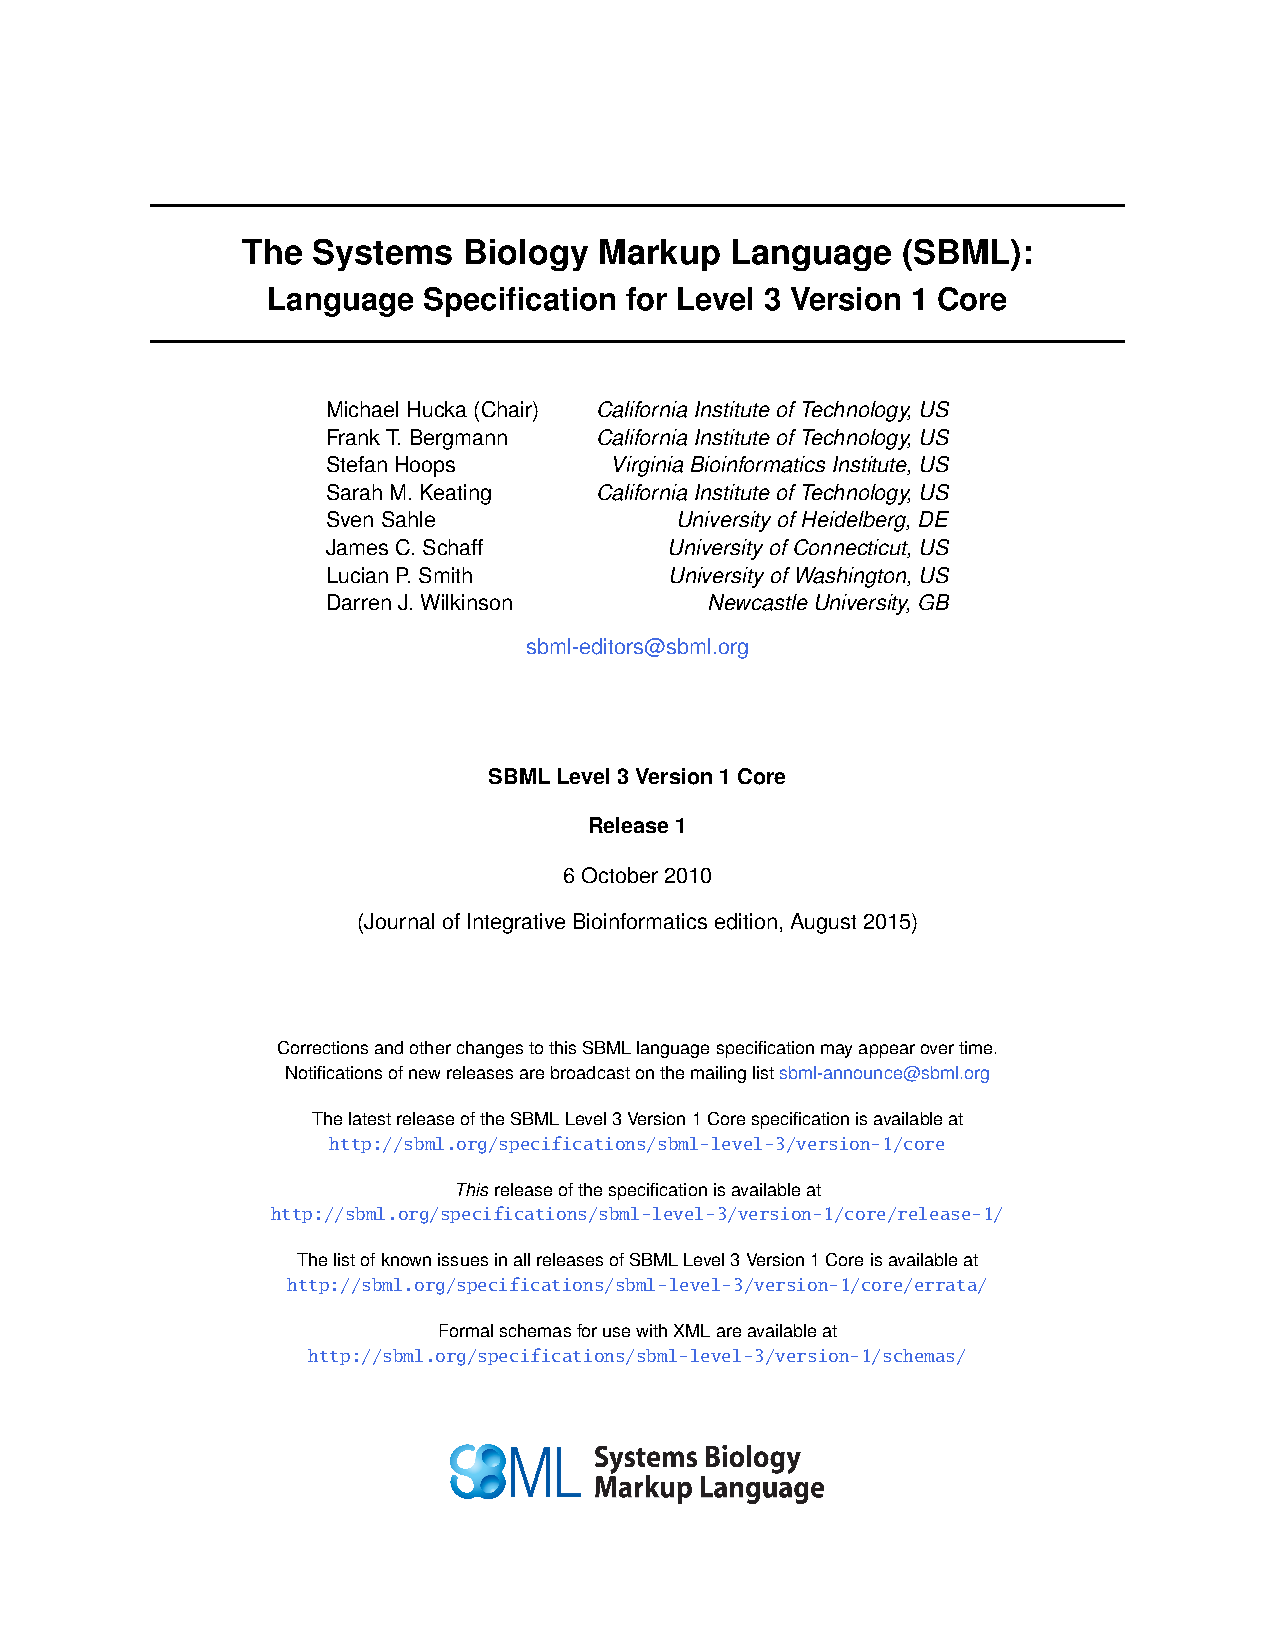
\includepdf[pages=-]{../spec/sbml-level-3-version-1-core.pdf}

\end{document}
